
%!TEX root = main.tex

\subsection{Semantics of $\LMAMASS$} \label{sect:semlmamass}

%We start with the semantics of $\LMAMASS$ and assume that $\Mm$ is an $\LMAMASS$. 

%Before presenting the formal semantics of $\LMAMASS$, let us describe the intuitions behind it.

%
\noindent\emph{Intuitions.}  We first explain the intuitions of the four launch modes. 

\begin{itemize}
	\item  $\STD$: When a new $\STD$-activity is started, it is pushed to the top task. 
	%
	\item $\STP$: When a new $\STP$-activity is started, if the activity is already at the top of the top task, it will reuse this activity. Otherwise, a new activity will be pushed into the top task.
	%
	\item $\STK$: When a new $\STK$-activity is started, it will create the activity at the root of a new task or locate the activity on an existing task with the same affinity. If the activity already exists, then all the activities above it are removed from the task. Otherwise, a new activity will be pushed into the task.
	%
	\item $\SIT$: 
	Similar to $\STK$, but if such an activity already exists, it will reuse this activity, moreover, there is only one activity in the task which was created by starting the same activity.
\end{itemize}




%Via extensive experiments, we identify a crucial notion, i.e., task affinity of tasks, which plays a pivotal role in such a mechanism.
When an activity is launched, it may not be put in the top task, in which case  
%When an activity $B$ is launched and not going to be put in the top task, 
the following rules are used to determine which task will it be allocated. 
\begin{itemize}
	\item In case $\lmd(B) \neq \SIT$, if there is a non-$\SIT$-task whose task affinity is the same as $B$, then $B$ will be put on the task; otherwise, a new task will be created to hold $B$.
	
	\item In case $\lmd(B) = \SIT$,    if there is any task whose bottom activity is $B$ (actually $B$ is the only activity in the task), then the task will be moved to the top; otherwise, a new task is created to hold $B$.
\end{itemize}

%%%%%%%%%%%%%%%%%%%%%%%%%%%%%%%%%%%%%%%%%%%%%%%
\noindent\textbf{Caveat.} The intuition is stated to facilitate readers to under the transitions rules at a high level. They are not necessarily precise at a formal level. For instance, when a new $\STD$-activity is stated by an $\SIT$-activity, the $\STD$-activity will not necessarily be pushed to the top task. 
%Task allocation mechanism is to specify to which task will it be allocated when an activity is launched. 
%%%%%%%%%%%%%%%%%%%%%%%%%%%%%%%%%%%%%%%%%%%%%%
%!TEX root = main.tex

We introduce some auxiliary functions and predicates to be used in the formal semantics of $\LMAMASS$.

%\begin{figure}
%	\begin{center}
	%\begin{tabular}{l}
	%\hline\\
	% $\topact(S) = A_1$, $\btmact(S) = A_m$\\
	%$\toptsk(\rho) = S_1$, $\topact(\rho) = \topact(\toptsk(\rho))$\\
	%$\push(\rho, B) = (([B]\cdot S_1,\aname_1),(S_2,\aname_2),\cdots,(S_n,\aname_n))$\\
	%\end{tabular}	
	%\caption{Auxiliary functions and predicates} \label{fig:syntax}
	%\end{center}
	%\end{figure}
	
	\paragraph{Auxiliary functions and predicates} 
	%To specify the transition relation precisely and concisely, we define the following functions and predicates. 
	Let $\rho= ((S_1,\aname_1),\cdots, (S_n,\aname_n))$ be a configuration and $S=[A_1, \cdots, A_m]$ be a task. 
	\begin{itemize}
		\item $\topact(S) = A_1$, $\btmact(S) = A_m$,
		\item $\toptsk(\rho) = S_1$, $\topact(\rho) = \topact(\toptsk(\rho))$, 
		\item $\push(\rho, B) = (([B]\cdot S_1,\aname_1),(S_2,\aname_2),\cdots,(S_n,\aname_n))$,
		\item $\Pop(\rho) = ((S_1',\aname_1),(S_2,\aname_2), \cdots, (S_n,\aname_n))$ if $S_1=[B]\cdot S_1'$ for some $B\in\act$ and $S_1'\in\act^+$,\\ $\Pop(\rho) = ((S_2,\aname_2),\cdots,(S_n,\aname_n))$ otherwise,
		% \item $\mvacttop(\rho, B) = ([B]\cdot S_1'\cdot S_1'', S_2, \cdots, S_n)$, if $S_1=S_1'\cdot[B]\cdot S_1''$ with $S_1'\in (\act\setminus\{B\})^*$,
		\item $\clrtop(\rho, B) = (([B]\cdot S_1'',\aname_1), (S_2,\aname_2), \cdots, (S_n,\aname_n))$, if $S_1=S_1'\cdot[B]\cdot S_1''$ with $S_1'\in (\act\setminus\{B\})^*$,
		% \item $\clrtsk(\rho, B) = ([B], S_2, \cdots, S_n)$,
		\item $\newtsk(\rho, B) = (([B],\aft(B)), S_1, \cdots, S_n)$,
		\item $\mvtsktop(\rho, i)$ is defined as 
		$$((S_i,\aname_i), (S_1,\aname_1), \cdots, (S_{i-1},\aname_{i-1}), (S_{i+1},\aname_{i+1}), \cdots, (S_n,\aname_n)),$$
		% \item $\gettsk(\rho, B) = S_i$ such that $i \in [n]$ is the \emph{minimum} index satisfying $\aft(A_i)=\aft(B)$, if such an index $i$ exists; $\gettsk(\rho, B) = *$ otherwise.
		%
		\item $\gettsk(\rho, B)$ is defined as follows,
		\begin{itemize}
			\item if $\lmd(B)\neq\singleinstance$, $\aname_i=\aft(B)$ and $\lmd(\btmact(S_i)) \neq \singleinstance$ for some $i \in [n]$,  then $\gettsk(\rho, B) = S_i$, otherwise, $\gettsk(\rho, B) = *$.
			\item if $\lmd(B) = \singleinstance$, $\btmact(S_i)=B$ for some $i \in [n]$, then $\gettsk(\rho, B) = S_i$, otherwise, $\gettsk(\rho, B) = *$.
		\end{itemize}
	\end{itemize}
	
Note that $\gettsk(\rho, B)$ formalizes the aforementioned task allocation mechanism and the fact that the task affinities of two different non-$\SIT$ tasks are distinct guarantees that the function $\gettsk(\rho, B)$ is well-defined. 
	
	%We are ready to define the semantics of $\LMAMASS$ as the transition relation $\xrightarrow[\Mm]{}$ in the sequel. 
	


\smallskip

\paragraph{Transition rules} 


Let $\rho = ((S_1,\aname_1),\cdots,(S_n,\aname_n))$ be the current configuration for some $n \ge 1$ and $\topact(\rho) = A$. Moreover, let $S_1 = [A_1',\cdots,A_m']$. Evidently, $A = A_1'$. We show how $\rho'$ can be obtained from $\rho$ and $\tau$.
	
	If $\tau = \back$, then $\rho' = \Pop(\rho)$. 
	
	Then consider $\tau = A\xrightarrow{\startactivity(\bot)}B$.
	
	% The definition of $\rho \xrightarrow[\Mm]{\tau} \rho'$ for $\tau= A\xrightarrow{\startactivity(\phi)}B$ is much more complicated. 
	% Let $\tau= A\xrightarrow{\startactivity(\phi)}B$ and $\rho = (S_1, \cdots, S_n)$ be the current configuration for some $n \ge 1$ such that $\topact(\rho) = A$. 
	% To ease the reading, we first consider the simpler cases that $\tau$ is from $\LMAMASS$ or $\IFAMASS$,  then consider the more general case that $\tau$ is from $\AMASS$. 
	
	
	% As the semantics of $\Mm$ are highly complex, we will formalize the semantics step by step. Firstly, we consider the case without the intent flag, then we consider the case with only the intent flag, and finally we consider the complete semantics.
	
	
	
	%\fcolorbox{red}{yellow}{%
		%	\minipage[t]{\dimexpr0.48\linewidth-2\fboxsep-2\fboxrule\relax}
		%	If $\lmd(A) \neq \SIT$, then $\rho'= \push(\rho,B)$.
		%	\endminipage}\hfill
	%\fcolorbox{red}{yellow}{%
		%	\minipage[t]{\dimexpr0.48\linewidth-2\fboxsep-2\fboxrule\relax}
		%	If $\lmd(A) = \SIT$, then
		%	\begin{itemize}
			%		\item if $\gettsk(\rho, B)=S_i$ for some $i\in[n]$,  then 
			%		$$\rho'=\push(\mvtsktop(\rho, i),B),$$
			%		\item if $\gettsk(\rho, B)=*$, then $\rho'= \newtsk(\rho,B )$.
			%	\end{itemize}
		%	\endminipage}
	
	
	\noindent \fbox{\fbox{$\lmd(B) = \STD$}}
	
	%\tcbset{width=(\linewidth-2mm)/2,before=,after=\hfill,arc=0mm,
		%	colframe=blue!75!black,colback=white,fonttitle=\bfseries}
	%title=Box \thetcbrasternum,
	%enhanced,size=small] %colframe=red!50!black,colback=red!10!white]
%	\begin{tcolorbox}[width=0.4\linewidth, title={$\lmd(A) = \SIT$}]
%		$\rho'= \push(\rho,B)$
%	\end{tcolorbox} \hfill
%	\begin{tcolorbox}[width=0.6\linewidth, title={$\lmd(A) \neq \SIT$}]
%		\begin{itemize}
%			\item if $\gettsk(\rho, B)=S_i$ for some $i\in[n]$,  then 
%			$\rho'=\push(\mvtsktop(\rho, i),B),$
%			\item	if $\gettsk(\rho, B)=*$, then $\rho'= \newtsk(\rho,B )$.
%		\end{itemize}
%	\end{tcolorbox}	
	
\begin{itemize}
				\item If $\lmd(A) \neq \SIT$, then $\rho'= \push(\rho,B)$.
				%
				\item If $\lmd(A) = \SIT$, then
		    		\begin{itemize}
			    			\item if $\gettsk(\rho, B)=S_i$ for some $i\in[n]$,  then 
						$$\rho'=\push(\mvtsktop(\rho, i),B),$$
			    			\item if $\gettsk(\rho, B)=*$, then $\rho'= \newtsk(\rho,B )$.
			    		\end{itemize}
\end{itemize}
	
	
	
	\noindent \fbox{\fbox{$\lmd(B) = \STP$}}
	\begin{itemize}
		\item  If $\lmd(A) \neq \SIT$ and $A \neq B$, then $\rho' = \push(\rho,B)$.
		%
		\item  If $\lmd(A) \neq \SIT$ and $A = B$, then $\rho' =  \rho$.
		%
		\item If $\lmd(A) = \SIT$, then
		\begin{itemize}
			\item if $\gettsk(\rho, B)=S_i$ for some $i\in[n]$,  then
			\begin{itemize}
				\item if $\topact(S_i)\neq B$, then 
				$$\rho'=\push(\mvtsktop(\rho, i),B),$$
				\item if $\topact(S_i)= B$, then $\rho'=\mvtsktop(\rho, i),$
			\end{itemize}
			\item if $\gettsk(\rho, B)=*$, then $\rho'= \newtsk(\rho,B )$.
		\end{itemize}
	\end{itemize}
	
	\noindent \fbox{\fbox{$\lmd(B) = \singletask$}}
	\begin{itemize}
		\item If $\gettsk(\rho, B) = S_i$ for some $i\in[n]$, then
		\begin{itemize}
			\item if $B \not \in S_i$, then $\rho' = \push(\mvtsktop(\rho, i), B)$,
			\item if $B  \in S_i$, 	then $\rho' =  \clrtop(\mvtsktop(\rho, i), B)$.
		\end{itemize}
		\item If $\gettsk(\rho, B) = *$, then $\rho' = \newtsk(\rho, B)$.
	\end{itemize}
	
	\noindent \fbox{\fbox{$\lmd(B) = \SIT$}}
	\begin{itemize}
		\item If $\gettsk(\rho, B) = S_i$ for some $i \in [n]$, then $\rho' = \mvtsktop(\rho, i)$.
		\item If $\gettsk(\rho, B) = *$, then $\rho' = \newtsk(\rho, B)$.
	\end{itemize}
	
	This concludes the definition of the transition rules for $\LMAMASS$. 
	
	
	
%	%%%%%%%%%%%%%%%%
%	\tl{to see where to put this.} Moreover, it is not hard to verify that the transition relation $\xrightarrow[\Mm]{\tau}$ preserves the invariant of configurations, that is, if $\rho$ satisfies that the task affinities of every two non-$\singleinstance$ tasks are different, and $\rho \xrightarrow[\Mm]{\tau} \rho'$ for some $\tau$, then $\rho'$ satisfies this invariant as well. 
%	%%%%%%%%%%%%%%%%%%%%%%

It is not hard to verify that the transition relation $\xrightarrow[\Mm]{}$ %preserves the invariant of configurations, that is, 
	satisfies that, if the task affinities of two non-$\singleinstance$ tasks are different in $\rho$ and $\rho \xrightarrow[\Mm]{\tau} \rho'$ for some $\tau$, then the task affinities of two non-$\singleinstance$ tasks are different in $\rho'$. 
	
	
	%%%%%%%%%%%%%%%%%%%%%%%%%%%%%%%%%%%%%%%%%% example %%%%%%%%%%%%%%%%%%%%%%%%%%%%%%%%%%%%%%%%%%%%%%%%
	We use the following example to illustrate the semantics.
	\begin{example}
		Let $\Mm = (\act,A,\lmd,\aft,\Delta)$ be an $\LMAMASS$, where $\act = \{A,B,C,D\}$, the functions $\lmd$ and $\aft$ are defined in Table~\ref{tab-attribute}.
		\begin{table}[htbp]
			\begin{center}
				\begin{tabular}{|c|c|c|c|c|c|}
					\hline
					Activity & $\lmd$ & $\aft$\\
					\hline
					$A$ & $\STD$ & 1 \\
					\hline
					$B$ & $\STK$ & 2 \\
					\hline
					$C$ & $\STP$ & 2 \\
					\hline
					$D$ & $\SIT$ & 3 \\
					\hline
				\end{tabular}
				\caption{Attributes of activities}
				\label{tab-attribute}
			\end{center}
		\end{table}
		
		Moreover, $\Delta = \{\back,\tau_1, \tau_2, \tau_3, \tau_4\}$, where 
		$\tau_1 = A \xrightarrow{\startactivity(\bot)} B$,
		$\tau_2 = B \xrightarrow{\startactivity(\bot)} C$,
		$\tau_3 = C \xrightarrow{\startactivity(\bot)} D$,
		$\tau_4 = D \xrightarrow{\startactivity(\bot)} B$,
		% $\tau_5 = D \xrightarrow{\startactivity(\bot)} C$.
		% $\rho_0 = (([D_1],D_1,1))$, and\\
		Then the configurations that are reachable from the initial configuration $(([A], 1))$ by executing the transition rules from $\Delta$ are illustrated in Figure~\ref{lmasm-example}, where the vertices denote the configurations and the edges denote the elements of $\xrightarrow[\Mm]{}$. 
		For instance, 
		\begin{itemize}
			\item if $A \xrightarrow{\startactivity(\bot)} B$ is applied to the configuration $(([A], 1))$, then a new task $([B],2)$ is created, since $\lmd(B) = \STK$ and $\gettsk((([A],1)), B) = *$, resulting in the configuration $(([B],2),([A],1))$,
			%
			% \item if $B \xrightarrow{\startactivity(\bot)} B$ is applied to the configuration $(([BA], 1))$, then $B$ will not be pushed, since $\lmd(B) = \STP$ and the top activity of the top task is $B$, 
			%
			\item if $B \xrightarrow{\startactivity(\bot)} C$ is applied to the configuration $(([B],2),([A],1))$, then $C$ is pushed, since $\lmd(C) = \STP$ and $B\neq C$, resulting in the configuration $(([CB],2),([A],1))$,
			%
			\item if $C \xrightarrow{\startactivity(\bot)} D$ is applied to the configuration $(([CB],2),([A],1))$, then a new task $([D], 3)$ is created, since 
			$$\lmd(D) = \SIT \mbox{ and } \gettsk((([CB],2),([A],1)), D) = *,$$ 
			resulting in the configuration $(([D],3),([CB],2),([A],1))$,
			%
			\item if $D \xrightarrow{\startactivity(\bot)} B$ is applied to the configuration $(([D],3),([CB],2),([A],1))$, then the task $([CB],2)$ is moved to the top and all the activities above $A$, which is $C$ here, are removed from the task, since $\lmd(B) = \STK$, 
			$$\gettsk((([D],3),([CB],2),([A],1)), B) = ([CB],2)$$
			and $B$ occurs in $([CB], 2)$, resulting in the configuration 
			$$(([B],2),([D],3),([A],1)),$$
			%
			% \item if $D \xrightarrow{\startactivity(\bot)} C$ is applied to the configuration $(([D],2),([CB],2),([A],1))$, then the task $([CB],2)$ is moved to the top, but $C$ will not be pushed, since $\lmd(C) = \STP$, $\lmd(D) = \SIT$,
			% $$\gettsk((([D],2),([CB],2),([A],1)), C) = ([CB],2)$$
			% and $C$ is the top activity of $([CB], 2)$, resulting in the configuration $(([CB],2),([D],2),([A],1))$,
			%
			\item if $C \xrightarrow{\startactivity(\bot)} D$ is applied to the configuration $(([CB],2),([D],3),([A],1))$, then the task $([D],3)$ is moved to the top, since $\lmd(D) = \SIT$ and
			$$\gettsk((([CB],2),([D],3),([A],1)), D) = ([D],3)$$
			resulting in the configuration $(([D],3),([CB],2),([A],1))$.
		\end{itemize}
		Note that for $\Mm$, there are only finitely many configurations reachable from the initial configuration, which may not be the case for $\LMAMASS$ in general.  
		% $(([D_1],D_1,1))$\\
		% $\xrightarrow[\tau_1]{\Mm}(([P_1D_1],D_1,1))$\\
		% $\xrightarrow[\tau_2]{\Mm}(([P_1D_1],D_1,1))$\\
		% $\xrightarrow[\tau_3]{\Mm}(([K_2],K_2,0),([P_1D_1],D_1,1))$\\
		% $\xrightarrow[\tau_4]{\Mm}(([D_1K_2],K_2,0),([P_1D_1],D_1,1))$\\
		% $\xrightarrow[\tau_5]{\Mm}(([T_2],T_2,0),([D_1K_2],K_2,0),([P_1D_1],D_1,1))$\\
		% $\xrightarrow[\tau_6]{\Mm}(([K_2],K_2,0),([T_2],T_2,0),([P_1D_1],D_1,1))$\\
		
		\begin{figure}
			% \vspace{-3mm}
			\centering
			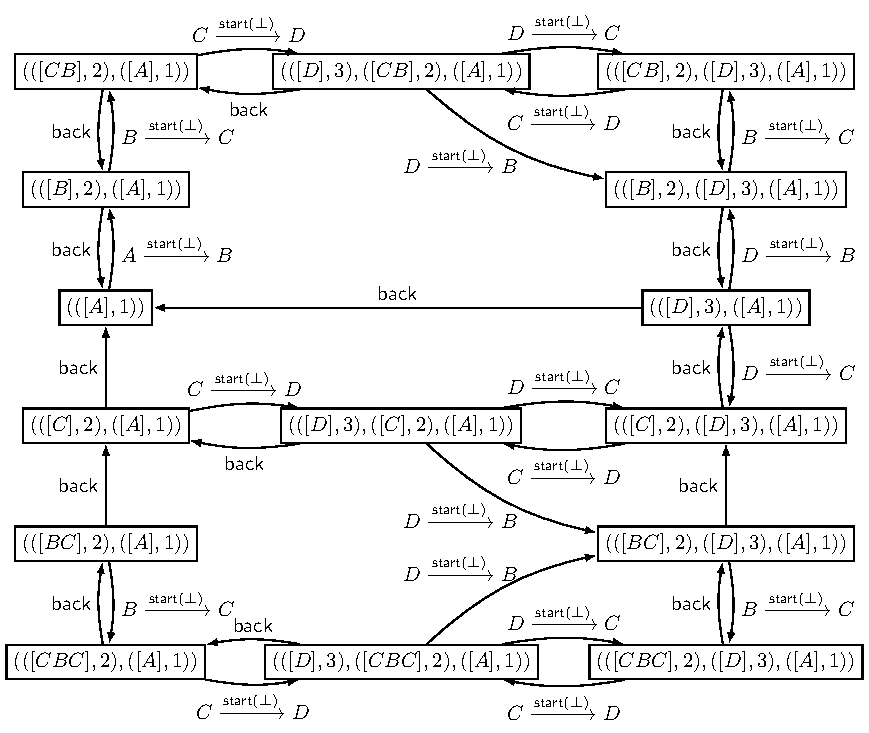
\includegraphics[scale = 1]{lmasm-example.pdf}
			\caption{Configurations reachable from the initial configuration $(([A], 1))$ in $\LMAMASS$}
			%in $\phi$
			% \vspace{-6mm}	
			\label{lmasm-example}
		\end{figure}
	\end{example}
	%%%%%%%%%%%%%%%%%%%%%%%%%%%%%%%%%%%%%%%%%%%%%%%%%%%%%% end of the example %%%%%%%%%%%%%%%%%%%%%%%%%%%%%%%%%%%%%%%%%
	% Intuitively, $\STD$ is similar to $\STP$, without considering the case where $\lmd(A) = \SIT$, when a $\STD$ activity $B$ is started, it is directly pushed into the top task. 
	% Recall that $\STP$ is shorthand of SingleToP, when a $\STP$ activity $B$ is started, it is pushed into the top task if the top activity of the top task is \emph{not} $B$.
	
	% $\SIT$ is similar to $\STK$, for each $\SIT$ (resp. $\STK$) activity $B$, it can appear at most once in the configuration. However, they still have differences. Recall that $\SIT$ is shorthand for SingleInsTance, that means the task which $\SIT$ activity located has only one activity. This also explains why starting an $\STD$ or $\STP$ activity, it is \emph{not} pushed into the current task when the callee activity is an $\SIT$ activity.
	% Moreover, when starting an activity $B$, if $\lmd(B)\in\{\STK,\SIT\}$ or the callee activity is the $\SIT$ activity, the first step is to specify to which task it will be allocated, more precisely, is to find the task which has the same task affinity with the caller activity. If the task is not found, it will launch a new task $[B]$ on the top of the configuration, if such a task $S_i$ is found, then $S_i$ will be moved to the top task of the configuration, and
	% \begin{itemize}
		% 	\item if $\lmd(B) = \STD$, then it will directly pushed into $S_i$,
		% 	\item if $\lmd(B) = \STP$, it is pushed into $S_i$ if the top activity of $S_i$ is \emph{not} $B$.
		% 	\item if $\lmd(B) = \SIT$, then $S_i$ will not change,
		% 	\item if $\lmd(B) = \STK$, then it will directly pushed into $S_i$ when $B\notin S_i$, it will poped until the top activity is $B$ otherwise,
		% \end{itemize}
